% !TeX root = main.tex
\chapter{Results and Discussion}\label{ch:results}
\section{Kinematic control}
In this section, we present the results of \vtwo{two} kinematic control simulation to demonstrate the effectiveness of the proposed vector field guidance strategy. \vtwo{The first simulation involves a system following a curve $\mathcal{C}$ in $\text{SE}(3)$, while the second simulation regards $\mathcal{C}$ in $\text{SO}^+(3, 1)$.} As the control is kinematic, the system follows a single integrator model
\begin{align}
    \dot{\mathbf{H}}(t) = \SL[\boldsymbol{\xi}(t)]\mathbf{H}(t),
\end{align}
where our control input is the generalized twist $\boldsymbol{\xi}$.
\subsection{Special Euclidean group}
The target curve $\mathcal{C}\subset\text{SE}(3)$ was based on a hyperbolic paraboloid rotating about the $x$-axis in the world frame. The parametrization of the curve $\mathbf{H}_d$ was defined as:
\begin{align}
    \mathbf{H}_d(s) = \begin{bmatrix}
        1 & \ \ 0 & 0 & r\cos(2\pi s)\\
        0 & \ \ \cos(2\pi s) & \sin(2\pi s) & r\sin(2\pi s)\\
        0 & -\sin(2\pi s) & \cos(2\pi s) & b + dr^2\bigl(\cos^2(2\pi s) - \sin^2(2\pi s)\bigr)\\
        0 & \ \ 0 & 0 & 1
    \end{bmatrix},
\end{align}
where $b=\qty{1}{\meter}$, $d=\qty{0.2}{\meter}$, and $r=\qty{1}{\meter}$. This curve was discretized into $P=\num{5000}$ points by sampling $s$ into $\num{5000}$ evenly spaced points within the interval $[0, 1]$. To distinguish the continuous and discrete parametrizations, we use the notations $\mathbf{H}_d[i]$ for the $i$-th sample of the discretized curve and $\mathbf{H}_d(s)$ for the continuous curve.
\subsubsection{Choice of S map}
For the simulation, we chose the canonical isomorphism $\SL$ between $\mathbb{R}^6$ and $\mathfrak{se}(3)$. Specifically, let $\boldsymbol{\xi} = [\xi_1 \ \xi_2 \ \xi_3 \ \xi_4 \ \xi_5 \ \xi_6]^\top$, the used $\SL$ is:
\begin{align}
    \SL[\boldsymbol{\xi}] = \begin{bmatrix}
    0 & -\xi_6 & \xi_5 & \xi_1 \\
    \xi_6 & 0 & -\xi_4 & \xi_2 \\
    -\xi_5 & \xi_4 & 0 & \xi_3 \\
    0 & 0 & 0 & 0
    \end{bmatrix}.
\end{align}
The basis $\mathbf{E}_1, ... ,\mathbf{E}_6$ of the Lie algebra $\mathfrak{se}(3)$ can be obtained by setting $\mathbf{E}_k = \SL[\mathbf{e}_k]$, where $\mathbf{e}_k$ are the columns of the $6 \times 6$ identity matrix. Geometrically, the interpretation of this basis choice is that $\boldsymbol{\xi}$ is the classical \emph{twist} in mechanics. More precisely, $\boldsymbol{\omega} \triangleq [\xi_4 \  \xi_5 \  \xi_6]^\top$ represents the $x$, $y$ and $z$-axes components of the angular  velocity  measured in the inertial frame, whereas $\mathbf{v} \triangleq [\xi_1 \  \xi_2 \  \xi_3]^\top$ represents the linear velocities, along the $x, y$ and $z$-axes, of a virtual point at the origin of the inertial frame, measured in this inertial frame. This is related to the object's linear velocity $\dot{\mathbf{p}}$  by $\dot{\mathbf{p}} = \boldsymbol{\omega} \times \mathbf{p} + \mathbf{v}$.

\subsubsection{Employed numerical methods}
To solve the optimization problem in \eqref{eq:optimization-problem-distance-definition-point-curve} and compute the distance $D(\mathbf{H})$, we used the discretized curve and computed the nearest point $\mathbf{H}_d[i^*]$ through a brute-force approach. Although it would be possible to compute the curve derivative explicitly, we opted for finite differences. Thus, we approximated the derivative $\mathbf{H}_d'[i]$ as
\begin{align}
    \mathbf{H}_d'[i] \approx \begin{cases}
        \frac{\mathbf{H}_d[i+1] - \mathbf{H}_d[i]}{\Delta s}, &  i < P\\    
        \frac{\mathbf{H}_d[1] - \mathbf{H}_d[i]}{\Delta s}, &  i = P,
    \end{cases}
\end{align}
adopting $\Delta s = \num{1E-3}$. This implies that our tangent component $\boldsymbol{\xi}_T$ is also approximate, since
\begin{align}
    \boldsymbol{\xi}_T \approx \invSL\biggl(\mathbf{H}_d'[i^*]\mathbf{H}_d[i^*]^{-1}\biggr).
\end{align}

For the computation of the normal component $\boldsymbol{\xi}_N$, we adopted an approximation by evaluating the right-hand side of \eqref{eq:Leq} for each $\mathbf{e}_i$. This gives the $i^{th}$ normal component element $\{\boldsymbol{\xi}_{N}\}_{i}$ as:
\begin{align}
    \{\boldsymbol{\xi}_{N}\}_{i} \approx \frac{\widehat{D}\Bigl(\exp\bigl(\SL[\boldsymbol{\mathbf{e}}_i]\bigr)\mathbf{H}(t), \mathbf{H}_d[s^*]\Bigr) - \widehat{D}\bigl(\mathbf{H}(t), \mathbf{H}_d[s^*]\bigr)}{\varepsilon},
\end{align} 
in which $\varepsilon = \num{1E-3}$ was used.

The system was simulated adopting the following approximation:
\begin{align}
    \mathbf{H}(t + \Delta t) \approx \exp\Bigl(\SL\bigl(\Psi(\mathbf{H})\bigr)\Delta t\Bigr)\mathbf{H}(t),
\end{align}
using a time step of $\Delta t = \qty{1E-2}{\second}$. 
\subsubsection{Vector field gains and initial condition}
The vector field gains were selected to complement each other, ensuring that the normal component would dominate when the system was far from the curve, and the tangent component would dominate when the system was near the curve. Based on this reasoning, the following gains were chosen:
\begin{align}
    k_N(\mathbf{H}) &= \tanh\bigl(20D(\mathbf{H})\bigr),\\
    k_T(\mathbf{H}) &= 1 - 0.5\tanh\bigl(D(\mathbf{H})\bigr).
\end{align}

The initial condition $\mathbf{H}(0)$ was set as
\begin{align}
    \mathbf{H}(0) = \begin{bmatrix}
        \frac{\sqrt{2}}{2} & -\frac{\sqrt{2}}{2} & 0 & -2\\
        \frac{\sqrt{2}}{2} & \ \frac{\sqrt{2}}{2} & 0 & -1\\
        0 & \ 0 & 1 & \ \ 0\\
        0 & \ 0 & 0 & \ 1
    \end{bmatrix}.
\end{align}
\subsubsection{Simulation}
\begin{figure}[ht!]
    \centering
    % First subfigure
    \begin{subfigure}[b]{0.32\textwidth}
        \centering
        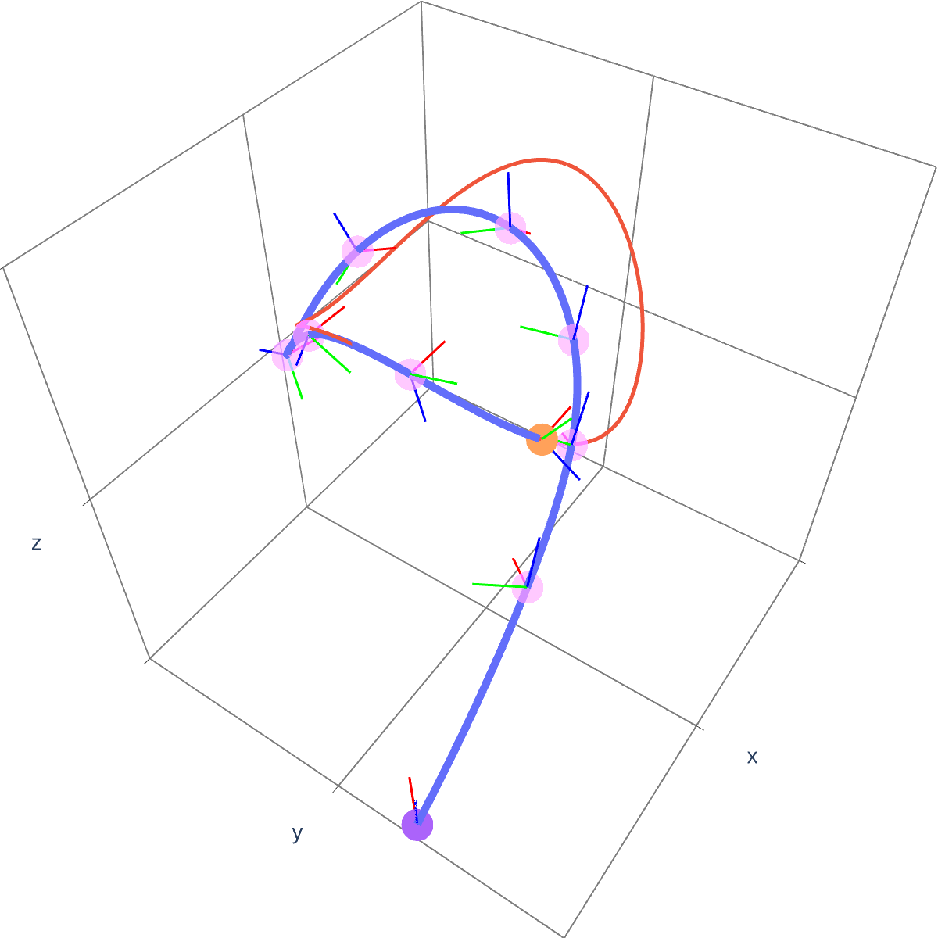
\includegraphics[width=\textwidth]{figures/vf_automatica_1.pdf} % Replace with your image
        \caption{$t\in[0, 5]s$}
        \label{fig:vfplot-first}
    \end{subfigure}
    \hfill
    % Second subfigure
    \begin{subfigure}[b]{0.32\textwidth}
        \centering
        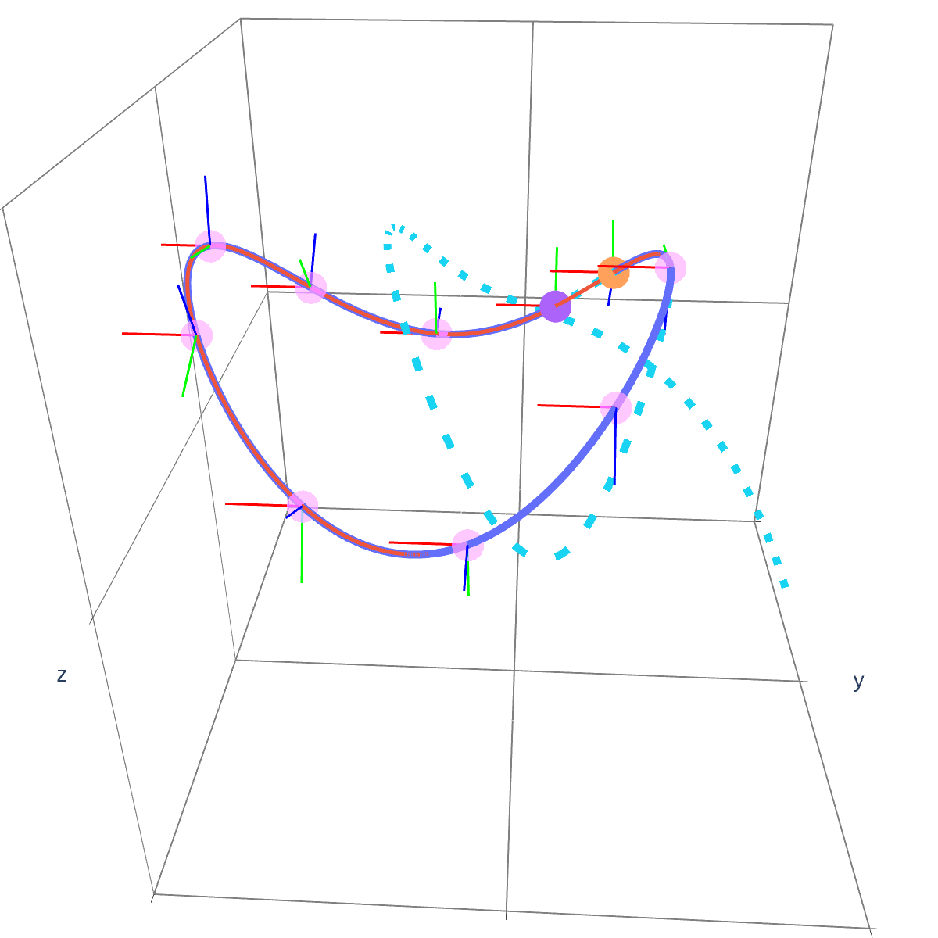
\includegraphics[width=\textwidth]{figures/vf_automatica_2.pdf} % Replace with your image
        \caption{$t\in[5, 9.7]s$}
        \label{fig:vfplot-second}
    \end{subfigure}
    \hfill
    % Third subfigure
    \begin{subfigure}[b]{0.32\textwidth}
        \centering
        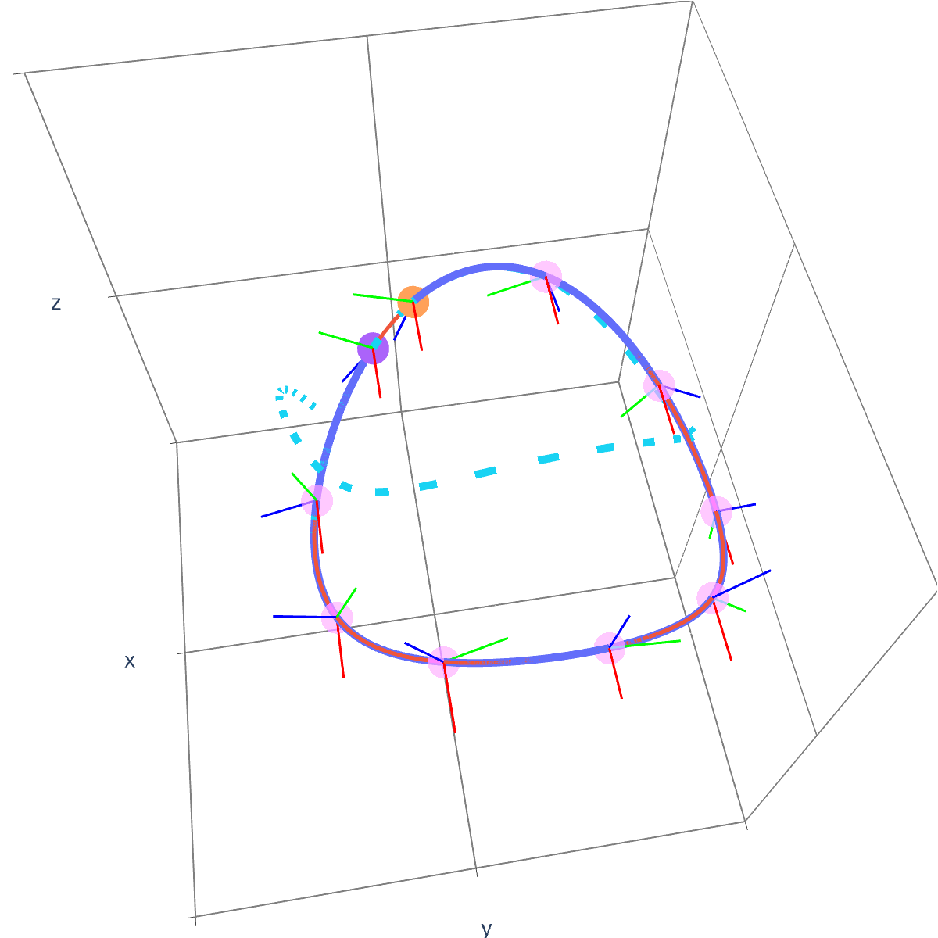
\includegraphics[width=\textwidth]{figures/vf_automatica_3.pdf} % Replace with your image
        \caption{$t\in[9.7, 14.5]s$}
        \label{fig:vfplot-third}
    \end{subfigure}
    \caption{The solid blue line depicts the system trajectory, while the solid red line indicates the target curve. The dashed light blue line represents the past trajectory. The initial and final positions are marked by purple and orange spheres, respectively. Translucent pink spheres denote intermediate positions, with orientation frames shown by RGB axes.}
    \label{fig:vfplot-trajectory}
\end{figure}
The simulation was conducted over a period of $\qty{15}{\second}$ and implemented in C++. On average, the computation of the vector field took $\qty{60 \pm 5}{\milli\second}$ per iteration on a single core of an Intel i5-10300H @ 4.5GHz CPU, with 8 GB of RAM. On average, $99.5\%$ of this time was spent solving the optimization problem in \eqref{eq:optimization-problem-distance-definition-point-curve}. Since the optimization process is highly parallelizable -- allowing simultaneous computation of $\widehat{D}(\mathbf{H},\mathbf{H}_d(s))$ for different discretized values of $s$ -- the computational effort could be significantly reduced by leveraging parallel architectures such as GPUs, SIMD, or multi-threading.
\begin{figure}[ht!]
    \centering
    \def\svgwidth{\linewidth}
    {\footnotesize\import{figures/}{distance_pos_ori_D.pdf_tex}}
    \caption{Value of EC-distance $D$, position error in centimeters and orientation error in degrees over time.}
    \label{fig:position-orientation-errors}
\end{figure}

The system's trajectory is illustrated in \cref{fig:vfplot-trajectory}, where the blue line represents the system trajectory, the red line represents the target curve, and the system state is depicted by colored spheres. The values of the distance function $D$ are shown in \cref{fig:position-orientation-errors}. Additionally, \cref{fig:position-orientation-errors} provides a more intuitive representation of the position error (in centimeters) and the orientation error (in degrees). These results confirm that the system successfully converges to the desired curve and circulates around it as expected. Once the system reaches the curve, it remains there without deviation. 

Although our implementation was carried out in C++, we provide a less efficient sample code in Python for clarity and accessibility, available at \url{https://github.com/fbartelt/SE3-example/blob/main/SE3example.ipynb}.
\subsection{Proper orthochronous Lorentz group}
\vtwo{Before describing the simulation conducted in $\text{SO}^+(3, 1)$, we first introduce key concepts from special relativity. Relativistic motion takes place within Minkowski space, a four-dimensional representation of spacetime. The elements of this space, known as \emph{events}, are represented by vectors $\mathbf{p}=[x\ y \ z\ t]^\top\in\mathbb{R}^4$, where $x$, $y$, and $z$ are spatial coordinates and $t$ is the time coordinate. Since effects such as time dilation and length contraction depend on the relative motion of observers, a transformation of reference frames is necessary to relate the coordinates of events between different observers. These transformations are known as \emph{Lorentz transformations}.}

\vtwo{Lorentz transformations form a group called the \emph{Lorentz group}, encompassing spatial rotations, reflections, and \emph{boosts} \citep[p. 12]{Carroll2019} -- the latter being transformations in Minkowski space without rotation, which are analogous to linear velocities in Minkowski space. Specifically, the proper orthochronous Lorentz group, $\text{SO}^+(3, 1)$, is a subgroup of the Lorentz group that includes only rotations and boosts preserving the direction of time. The elements of $\text{SO}^+(3, 1)$ are $4 \times 4$ matrices that preserve the \emph{Minkowski metric}, defined by:}
\vtwo{
\begin{align}
    \nu^2 = x^2 + y^2 + z^2 - c^2t^2, \label{eq:results-lorentz-metric}
\end{align}
where $\nu$ is the \emph{spacetime interval}, and $c$ is the speed of light.}

\vtwo{If an observer $O_2$ moves near the speed of light, they will perceive an event with coordinates $\mathbf{p}' = [x'\ y'\ z'\ t']^\top$ that differ from the coordinates $\mathbf{p}$ observed by an inertial observer $O_1$. These coordinates are related by the transformation $\mathbf{p}' = \boldsymbol{\Lambda} \mathbf{p}$, where $\boldsymbol{\Lambda}$ is a Lorentz transformation. For instance, if $O_2$ moves along the $x$-axis with velocity $v$, the Lorentz transformation is given by
\begin{align}
   \begin{split}
     x' &= \gamma(x - vt),\\
     y' &= y,\\
     z'&=z,\\
     t' &= \gamma\Bigl(t - \frac{vx}{c^2}\Bigr),\label{eq:results-lorentz-example}
   \end{split}
\end{align}
where $\gamma = \frac{1}{\sqrt{1 - v^2/c^2}}$ is the \emph{Lorentz factor}.}

\vtwo{As shown in \eqref{eq:results-lorentz-example}, observer $O_2$ experiences time dilation when traveling near the speed of light. It is common to interpret the differing ``times'' as if each reference frame has an attached clock that ticks at a distinct rate. The time measured by a clock in the inertial frame $O_1$ is referred to as the \emph{coordinate time}, while the time measured by a clock in the relativistic frame $O_2$ is called the \emph{proper time}. The proper time $\tau$ is related to the coordinate time $t$ via $\frac{dt}{d\tau} = \gamma$ \citep[p. 32]{steane2012relativity}.}

\vthree{Although there exists a physical meaning for this group, we only use it as a mathematical structure in our simulation. As such, we do not provide any interpretation for the curve following behavior. The equations shown are valid for non-varying boosts along one axis, however, the general case is more complex and would require a more thorough analaysis. While the curve was constructed in a simple way, the motion generated by the vector field might induce both spatial rotations and boosts along any direction.}

% To ensure dimensionality consistency, it is usual to adopt $c = 1$ in special relativity, implying that all quantities are dimensionless. This approach was also adopted in our simulation.

% \vthree{The usage of $ct$ can be substituted by a simple change in $\mathbf{I}_{3,1}$ of \cref{ex:indefinite-orthogonal-group-lorentz-group}. First note that for a vector $\mathbf{p}=[x\ y \ z\ t]^\top$, the metric \eqref{eq:results-lorentz-metric} can be represented as $\mathbf{p}^\top\boldsymbol{\Theta}\mathbf{p}$, where
% \begin{align}
%     \boldsymbol{\Theta} = \begin{bmatrix}
%         \mathbf{I} & \mathbf{0}\\
%         \mathbf{0} & -c
%     \end{bmatrix}.
% \end{align}
% Since this metric is preserved through Lorentz transformations $\boldsymbol{\Lambda}$, we have
% \begin{align}
%     \begin{split}
%         \mathbf{p}^\top\boldsymbol{\Theta}\mathbf{p} &= (\mathbf{p}')^\top\boldsymbol{\Theta}\mathbf{p}' = \mathbf{p}^\top\bigl(\boldsymbol{\Omega}^\top\boldsymbol{\Theta}\boldsymbol{\Omega}\bigr)\mathbf{p}\\
%         \implies \boldsymbol{\Theta} &= \boldsymbol{\Omega}^\top\boldsymbol{\Theta}\boldsymbol{\Omega},
%     \end{split}
% \end{align}
% which is equivalent to the definition of the group (\cref{ex:indefinite-orthogonal-group-lorentz-group}) with a modified $\mathbf{I}_{3,1}$.} 

% \vthree{Based in this modification, we now study the Lie algebra $\mathfrak{so}(3,1)$. To achieve the format in \cref{ex:lorentz-group-lie-algebra}, and element $\mathbf{A}\in\mathfrak{so}(3,1)$ must obey the following relation \citep[p. 59]{Hall2015}:
% \begin{align}
%     \boldsymbol{\Theta}\mathbf{A} &= -\mathbf{A}^\top\boldsymbol{\Theta}\\
%     \begin{bmatrix}
%         \mathbf{I} & \mathbf{0}\\
%         \mathbf{0} & -c
%     \end{bmatrix}\begin{bmatrix}
%         \mathbf{B} & \mathbf{a}\\
%         \mathbf{b}^\top & d
%     \end{bmatrix} &= \begin{bmatrix}
%         \mathbf{B}^\top & \mathbf{b}\\
%         \mathbf{a}^\top & d
%     \end{bmatrix}\begin{bmatrix}
%         -\mathbf{I} & \mathbf{0}\\
%         \mathbf{0} & c
%     \end{bmatrix}\\
%     \begin{bmatrix}
%         \mathbf{B} & \mathbf{a}\\
%         -c\mathbf{b}^\top & -cd
%     \end{bmatrix} &= \begin{bmatrix}
%         -\mathbf{B}^\top & c\mathbf{b}\\
%         -\mathbf{a}^\top & cd
%     \end{bmatrix},
% \end{align}
% which implies that $\mathbf{B}$ is skew-symmetric, $d$ is zero, and $a=c\mathbf{b}$. Thus, an element $\mathbf{A}\in\mathfrak{so}(3,1)$ can be represented as
% \begin{align}
%     \mathbf{A} = \begin{bmatrix}
%         \mathbf{B} & \mathbf{a}\\
%         \frac{1}{c}\mathbf{a}^\top & 0
%     \end{bmatrix}\in\mathbb{R}^{4\times 4}, \ \mathbb{R}^{3\times3}\ni\mathbf{B} = -\mathbf{B}^\top, \mathbf{a}\in\mathbb{R}^3. \label{eq:results-equation-lorentz-ref}
% \end{align}
% }

% \vthree{Using the format in \eqref{eq:results-equation-lorentz-ref}, we note that for boosts $\mathbf{a}$ with magnitude much smaller than the speed of light, the term $\frac{1}{c}\mathbf{a}^\top$ tends to zero. This is exactly the Lie algebra $\mathfrak{se}(3)$, which shows that $\mathfrak{se}(3)$ is a particular case of $\mathfrak{so}(3,1)$. This further implies that the Lie group $\text{SE}(3)$ is a particular case of $\text{SO}^+(3,1)$, which is expected since motions with ``low'' velocities obey Newtonian mechanics. This result also shows that the concept of boosts in special relativity is a generalization of linear velocities in classical mechanics.}

\vtwo{With these concepts established, we now turn to the simulation conducted in $\text{SO}^+(3, 1)$. For simplicity, we adopt $c = 1$, as is customary in special relativity, implying all quantities are dimensionless.}

\subsubsection{Target curve}
\vtwo{The target curve $\mathcal{C} \subset \text{SO}^+(3, 1)$ was chosen as a periodic boost along the $x$-axis. The parametrization of the curve, denoted by $\mathbf{H}_d$, is defined as:
\begin{align}
    \mathbf{H}_d(s) = \begin{bmatrix}
        \gamma(s) & 0 & 0 & -\gamma(s) v(s)\\
        0 & 1 & 0 & 0\\
        0 & 0 & 1 & 0\\
        -\gamma(s) v(s) & 0 & 0 & \gamma(s)
    \end{bmatrix},\label{eq:results-lorentz-curve-parametrization}
\end{align}
where
\begin{align}
    v(s) &= 0.9 + \frac{0.09}{2}(\cos(2\pi s) + 1),\\
    \gamma(s) &= \frac{1}{\sqrt{1 - v(s)^2}}.
\end{align}}
\vtwo{This curve was discretized into $P=\num{30000}$ points by sampling $s$ into $\num{30000}$ evenly spaced points within the interval $[0, 1]$. To distinguish the continuous and discrete parametrizations, we again adopt the notations $\mathbf{H}_d[i]$ for the $i$-th sample of the discretized curve and $\mathbf{H}_d(s)$ for the continuous curve.}

\subsubsection{Choice of S map}
\vtwo{The selected S map is the same as the one presented in \cref{ex:lorentz-group-lie-algebra}. Thus, for a vector $\boldsymbol{\xi}=[\xi_1\ \xi_2\ \xi_3\ \xi_4\ \xi_5\ \xi_6 ]^\top$, the corresponding isomorphism $\mathcal{S}:\mathbb{R}^6\to\mathfrak{so}(3,1)$ is given by:
\begin{align}
    \SL[\boldsymbol{\xi}] = \begin{bmatrix}
        0 & -\xi_3 & \xi_2 & \xi_4 \\
        \xi_3 & 0 & -\xi_1 & \xi_5 \\
        -\xi_2 & \xi_1 & 0 & \xi_6 \\
        \xi_4 & \xi_5 & \xi_6 & 0
    \end{bmatrix}.
\end{align}}
\subsubsection{Employed numerical methods}
\vtwo{The optimization problem in \eqref{eq:optimization-problem-distance-definition-point-curve} was solved using the discretized curve, with the nearest point $\mathbf{H}_d[i^*]$ computed through a brute-force approach. The derivative $\mathbf{H}_d'[i]$ was obtained as the explicit derivative of the discrete version of \eqref{eq:results-lorentz-curve-parametrization}. The normal component was approximated following the same method as in the previous simulation. Specifically, the $i^{th}$ normal component element $\{\boldsymbol{\xi}_{N}\}_{i}$ as:
\begin{align}
    \{\boldsymbol{\xi}_{N}\}_{i} \approx \frac{\widehat{D}\Bigl(\exp\bigl(\SL[\boldsymbol{\mathbf{e}}_i]\bigr)\mathbf{H}(t), \mathbf{H}_d[s^*]\Bigr) - \widehat{D}\bigl(\mathbf{H}(t), \mathbf{H}_d[s^*]\bigr)}{\varepsilon},
\end{align} 
in which $\varepsilon = \num{1E-5}$ was used.}

\vtwo{The system was also simulated adopting the same approximation
\begin{align}
    \mathbf{H}(t + \Delta t) \approx \exp\Bigl(\SL\bigl(\Psi(\mathbf{H})\bigr)\Delta t\Bigr)\mathbf{H}(t),
\end{align}
using a time step of $\Delta t = \qty{1E-3}{\second}$.}
\subsubsection{Vector field gains and initial condition}
\vtwo{The gains were selected following the same reasoning as in the previous simulation, ensuring that the normal component would dominate when the system was far from the curve, while the tangent component would dominate when the system was near the curve. The chosen gains were:
\begin{align}
    k_N(\mathbf{H}) &= \tanh\bigl(\num{1000}D(\mathbf{H})\bigr)\\
    k_T(\mathbf{H}) &= 0.5\Bigl(1 - \tanh\bigl(100D(\mathbf{H})\bigr)\Bigr).
\end{align}}

\vtwo{The initial condition $\mathbf{H}(0)$ was set as a boost along the $x$-axis in the opposite direction:
\begin{align}
    \mathbf{H}(0) = \exp\bigl(\SL[\boldsymbol{\xi}_0]\bigr),
\end{align}
where $\boldsymbol{\xi}_0 = [0\ 0\ 0\ 0.7\ 0\ 0]^\top$.}
\subsubsection{Simulation}
\begin{figure}[ht!]
    \centering
    \def\svgwidth{\linewidth}
    {\footnotesize\import{figures/}{lorentz_distanceD.pdf_tex}}
    \caption{Value of EC-distance $D$ in $\text{SO}^+(3,1)$ over time.}
    \label{fig:lorentz-sim-distance-D}
\end{figure}
\vthree{As it is unfeasible to plot the behavior of the system in $\text{SO}^+(3, 1)$ directly, we can only provide the value of the distance function along the simulated time, which is shown in \cref{fig:lorentz-sim-distance-D}. The system successfully converges to the desired curve, achieving a final distance of approximately $0.02$, which was deemed acceptable but could potentially be reduced by adjusting} \vthree{$\varepsilon$ in the approximation of the normal component. Although slowly, the magnitude of the distance is decreasing along the interval shown.} 
% \begin{figure}[ht!]
%     \centering
%     \def\svgwidth{\linewidth}
%     {\footnotesize\import{figures/}{lorentz_inert_mov.pdf_tex}}
%     \caption{Circular motion with respect to the inertial frame along its coordinate time, and the perceived motion in the relativistic frame along its proper time.}
%     \label{fig:lorentz-sim-inertial-motion}
% \end{figure}

% \vtwo{The first visualization is shown in \cref{fig:lorentz-sim-inertial-motion}, where we set $\mathbf{p}=\mathbf{p}_c$, which represents a circular motion with respect to the inertial frame, and $\mathbf{p}'=\mathbf{H}(t)\mathbf{p}$ denotes the motion as perceived by the relativistic observer. The elapsed proper time was computed as $\Delta \tau = \frac{1}{\gamma}\Delta t$. As shown, an observer following the system's motion -- continuously transitioning between referential frames -- perceives a distorted circular trajectory. At maximum speed, the proper elapsed time for this observer is approximately $40\%$ of the coordinate elapsed time.}
% \begin{figure}[ht!]
%     \centering
%     \def\svgwidth{\linewidth}
%     {\footnotesize\import{figures/}{lorentz_relat_mov.pdf_tex}}
%     \caption{Circular motion with respect to the relativistic frame along its proper time, and the perceived motion in the inertial frame along its coordinate time.}
%     \label{fig:lorentz-sim-relativistic-motion}
% \end{figure}

% \vtwo{The second visualization is shown in \cref{fig:lorentz-sim-relativistic-motion}, where $\mathbf{p}'=\mathbf{p}_c$ represents a circular motion in the relativistic frame, and $\mathbf{p}=\mathbf{H}^{-1}(t)\mathbf{p}'$ denotes the motion as perceived in the inertial frame. The elapsed coordinate time is computed as $\Delta t = \gamma\Delta\tau$. As observed, an inertial frame observer perceives the system's motion as a distorted circular trajectory, albeit distinct from the one seen by the relativistic observer. The elapsed time further indicates that events in the inertial frame occur at a slower rate, with the coordinate elapsed time being nearly double the proper elapsed time.}
% \begin{figure}[ht!]
%     \centering
%     \def\svgwidth{\linewidth}
%     {\footnotesize\import{figures/}{lorentz_time_dilat.pdf_tex}}
%     \caption{Effect of time dilation on the perceived time in the relativistic frame (proper time) and the inertial frame (coordinate time).}
%     \label{fig:lorentz-sim-time-dilat}
% \end{figure}

% \vtwo{A comparison of both the proper time and the coordinate time is shown in \cref{fig:lorentz-sim-time-dilat}. As observed, the proper time elapses slower than the coordinate time due to the effect of time dilation, a fundamental consequence of special relativity. This effect becomes increasingly pronounced as the system approaches the speed of light, consistent with theoretical expectations.}


% \vtwo{Finally, the value of the EC-distance $D$ is shown in }

\section{Collaborative Manipulation}
For the adaptive control simulation described in \cref{ch:collaborative}, we considered the manipulation of a large cylindrical body by six agents. The goal was to converge to and circulate a curve $\mathcal{C}\subset\mathbb{R}^3\times\text{SO}(3)$. The cylindrical body had a radius $r$ of $\qty{0.25}{\meter}$, a height $h$ of $\qty{1}{\meter}$, and a mass $m$ of $\qty{1.28E3}{\kilogram}$. The measurement point $\mathbf{r}_p$ was taken as the position of the first agent, $\mathbf{r}_1=[0\ 0\ 1.5]^\top$. The positions of the other agents, along with the components of the inertia tensor, are provided in \cref{tb:parameters}.
\begin{table}[htb]
    \centering
    \begin{threeparttable}
    \caption{Adaptive simulation parameters}\label{tb:parameters}
    \begin{tabular}{clcl}
    Parameter & Value & Parameter & Value\\\hline
    $r$ & $\qty{0.25}{\meter}$ & $\mathbf{r}_{1}$ & $[0\ 0\ 1.5]^\top\,\unit{\meter}$\\
    $h$ & $\qty{1}{\meter}$ & $\mathbf{r}_{2}$ & $[0\ 0\ -1.5]^\top\,\unit{\meter}$\\
    $m$ & $\qty{1.28E3}{\kilogram}$ & 
    $\mathbf{r}_{3}$ & $[0.5\ 0\ 0]^\top\,\unit{\meter}$\\
    $\mathbb{I}_{\text{cm}, xx}$ & $\qty{1.56E2}{\kilogram\meter\squared}$ & 
    $\mathbf{r}_{4}$ & $[-0.5\ 0\ 0]^\top\,\unit{\meter}$\\  
    $\mathbb{I}_{\text{cm}, yy}$ & $\qty{1.56E2}{\kilogram\meter\squared}$ &
    $\mathbf{r}_{5}$ & $[0\ 0.5\ 0]^\top\,\unit{\meter}$\\
    $\mathbb{I}_{\text{cm}, zz}$ & $\qty{4.93E1}{\kilogram\meter\squared}$  & 
    $\mathbf{r}_{6}$ & $[0\ -0.5 \ 0]^\top\,\unit{\meter}$\\
    $\mathbf{r}_{p}$ & $[0\ 0\ 1.5]^\top\,\unit{\meter}$ \\\hline
    \end{tabular}
    \begin{tablenotes}
        \footnotesize
        \item Note: The inertia tensor $\mathbb{I}_\text{cm}$ is diagonal, with the components $\mathbb{I}_{\text{cm}, xx}, \mathbb{I}_{\text{cm}, yy}$ and $\mathbb{I}_{\text{cm}, zz}$ representing the diagonal elements in order.
    \end{tablenotes}
    \end{threeparttable}
\end{table}

\subsection{Curve parametrization and S map}
In this simulation, we employed a more complex curve in the group $\text{ISE}(3)$, defined as:
\begin{align}
    \mathbf{H}_d(s) = \begin{bmatrix}
        \mathbf{R}_d(s) & \mathbf{0} & \mathbf{0}\\
        \mathbf{0} & \mathbf{I} & \mathbf{p}_d(s)\\
        \mathbf{0} & \mathbf{0} & 1
    \end{bmatrix},\label{eq:parametriceq-simulation}
\end{align}
where
\begin{align}
    \mathbf{p}_d(s) &= \begin{bmatrix}
        0.7(\sin(2\pi s) + 2\sin(4\pi s))\\
        0.7(\cos(2\pi s) - 2\cos(4\pi s))\\
        0.4 - 0.7\sin(6\pi s)
    \end{bmatrix},\\
    \mathbf{R}_d(s) &= \begin{bmatrix}
        \cos(2\pi s) & -\sin(2\pi s) & 0\\
        \sin(2\pi s) & \cos(2\pi s) & 0\\
        0 & 0 & 1
    \end{bmatrix}\begin{bmatrix}
        1 & 0 & 0\\
        0 & \cos(4\pi s) & -\sin(4\pi s)\\
        0 & \sin(4\pi s) & \cos(4\pi s)
    \end{bmatrix}.
\end{align}
Instead of using the continuous curve, we discretized it into $P=\num{2000}$ points by sampling the parameter $s$ into $\num{2000}$ evenly spaced values within the interval $[0, 1]$. To distinguish between the discrete and continuous representations, we henceforth use the notations $\mathbf{H}_d[i]$, $\mathbf{p}_d[i]$ and $\mathbf{R}_d[i]$ to refer to the $i^{th}$ sample of the curve, position and orientation, respectively.

\vthree{We selected the following S map for a vector $\boldsymbol{\xi}=[\xi_1\ \xi_2\ \xi_3\ \xi_4\ \xi_5\ \xi_6]^\top=[\mathbf{v}^\top\ \boldsymbol{\omega}^\top]^\top$, where $\mathbf{v},\boldsymbol{\omega}\in\mathbb{R}^3$:
\begin{align}
    \SL[\boldsymbol{\xi}] = \begin{bmatrix}
        \widehat{\mathcal{S}}(\boldsymbol{\omega}) & \mathbf{0} & \mathbf{0}\\
        \mathbf{0} & \mathbf{0} & \mathbf{v}\\
        \mathbf{0} & \mathbf{0} & 0
    \end{bmatrix},
\end{align}
where $\widehat{\mathcal{S}}$ is the canonical isomorphism for $\mathfrak{so}(3)$ (see \cref{ex:orthogonal-group-special-orthogonal-group-lie-algebra}).}
\subsection{Employed numerical methods}\label{sec:results-adaptive-nummerical-methods}
Although the curve is represented in $\text{ISE}(3)$, our adaptive control formulation used the tuple representation of $\mathbb{R}^3\times \text{SO}(3)$. To avoid confusion, we use $\mathbf{H}$ to represent the element of $\text{ISE}(3)$ and $\boldsymbol{\chi}=(\mathbf{R}, \mathbf{p})$ to represent the same entity as an element of $\mathbb{R}^3\times \text{SO}(3)$. This equivalence implies that $\boldsymbol{\xi}=\dot{\boldsymbol{\chi}}$ and $\dot{\boldsymbol{\xi}} = \ddot{\boldsymbol{\chi}}$, thus we adopt the notation using $\boldsymbol{\chi}$ for twists and accelerations to maintain consistency with the dynamics outlined in \cref{sec:dynamic-modelling}.

The reference model, as defined in \eqref{eq:ref-model-linear-parametrization}, depends on the acceleration, which is the derivative of the vector field. This acceleration was approximated using the symmetric difference quotient: 
\begin{align}
    \dot{\Psi}\bigl(\mathbf{H}(t)\bigr) \approx \frac{\Psi\Biggl(\exp\biggl(\SL\Bigl(\Delta t\Psi\bigl(\mathbf{H}(t)\bigr)\Bigr)\biggr)\mathbf{H}(t)\Biggr) - \Psi\Biggl(\exp\biggl(\SL\Bigl(-\Delta t\Psi\bigl(\mathbf{H}(t)\bigr)\Bigr)\biggr)\mathbf{H}(t)\Biggr)}{2\Delta t}. \label{eq:approximation-derivative-psi}
\end{align}

We then discuss the integration of the system using \emph{Heun's method} \citep[p. 330]{fred2007algoritmos}, also known as the \emph{improved Euler method}, which is a two-stage Runge-Kutta method. To describe how this method was applied in the context of Lie groups, we use the notation $\underline{\cdot}$ for the intermediate variables in Heun's method. Let $\mathbf{H}_\text{ref}$ denote the reference state, i.e., the state of the system if it were following the vector field perfectly. The update for the system's acceleration $\ddot{\boldsymbol{\chi}}$, the derivatives of the parameters $\dot{\widehat{\mathbf{o}}}_i$ and $\dot{\widehat{\mathbf{r}}}_i$, and the respective intermediate variables were taken as follows:
\begin{align}
    \begin{split}
        \ddot{\underline{\boldsymbol{\chi}}}(t+\Delta t) &= \mathbf{M}\bigl(\underline{\boldsymbol{\chi}}(t)\bigr)^{\dagger(\epsilon)}\biggl(-\mathbf{C}\bigl(\underline{\boldsymbol{\chi}}(t), \underline{\dot{\boldsymbol{\chi}}}(t)\bigr)\underline{\dot{\boldsymbol{\chi}}}(t)  + \sum_{i=1}^6 \mathbf{G}\bigl(\underline{\boldsymbol{\chi}}(t), \underline{\widehat{\mathbf{r}}}_i(t)\bigr)^{-1}\underline{\boldsymbol{\eta}}_i(t)\biggr),\\
        \ddot{{\boldsymbol{\chi}}}(t+\Delta t) &= \mathbf{M}\bigl({\boldsymbol{\chi}}(t)\bigr)^{\dagger(\epsilon)}\biggl(-\mathbf{C}\bigl({\boldsymbol{\chi}}(t), {\dot{\boldsymbol{\chi}}}(t)\bigr)\dot{\boldsymbol{\chi}}(t)  + \sum_{i=1}^6 \mathbf{G}\bigl({\boldsymbol{\chi}}(t), {\widehat{\mathbf{r}}}_i(t)\bigr)^{-1}{\boldsymbol{\eta}}_i(t)\biggr),\\
        \underline{\dot{\widehat{\mathbf{o}}}}_i(t + \Delta t) &= -\boldsymbol{\Gamma}_o\mathbf{Y}_o\Bigl(\underline{\boldsymbol{\chi}}(t), \underline{\dot{\boldsymbol{\chi}}}(t), \Psi\bigl(\underline{\mathbf{H}}_\text{ref}(t)\bigr), \dot{\Psi}\bigl(\underline{\mathbf{H}}_\text{ref}(t)\bigr)\Bigr)\underline{\boldsymbol{\zeta}},\\
        {\dot{\widehat{\mathbf{o}}}}_i(t + \Delta t) &= -\boldsymbol{\Gamma}_o\mathbf{Y}_o\Bigl({\boldsymbol{\chi}}(t), {\dot{\boldsymbol{\chi}}}(t), \Psi\bigl({\mathbf{H}_\text{ref}}(t)\bigr), \dot{\Psi}\bigl({\mathbf{H}_\text{ref}}(t)\bigr)\Bigr){\boldsymbol{\zeta}},\\
        \underline{\dot{\widehat{\mathbf{r}}}}_i(t + \Delta t) &= -\boldsymbol{\Gamma}_r\mathbf{Y}_r\bigl(\underline{\boldsymbol{\eta}}_i(t), \underline{\boldsymbol{\chi}}(t)\bigr)\underline{\boldsymbol{\zeta}},\\
        \underline{\dot{\widehat{\mathbf{r}}}}_i(t + \Delta t) &= -\boldsymbol{\Gamma}_r\mathbf{Y}_r\bigl({\boldsymbol{\eta}}_i(t), {\boldsymbol{\chi}}(t)\bigr){\boldsymbol{\zeta}},
    \end{split}
\end{align}
where $\underline{\boldsymbol{\eta}}_i(t) = \mathbf{Y}_o\Bigl(\underline{\boldsymbol{\chi}}(t), \underline{\dot{\boldsymbol{\chi}}}(t), \Psi\bigl(\underline{\mathbf{H}}_\text{ref}(t)\bigr), \dot{\Psi}\bigl(\underline{\mathbf{H}}_\text{ref}(t)\bigr)\Bigr)\underline{\widehat{\mathbf{o}}}_i(t) - \mathbf{K}_D\underline{\boldsymbol{\zeta}}$, the intermediate velocity error $\underline{\boldsymbol{\zeta}}$ is given by $\underline{\boldsymbol{\zeta}}=\underline{\dot{\boldsymbol{\chi}}}(t) - \Psi\bigl(\underline{\mathbf{H}}_\text{ref}(t)\bigr)$, and $\mathbf{M}^{\dagger(\epsilon)}$ is the damped pseudo-inverse $\mathbf{M}^{\dagger(\epsilon)} = (\mathbf{M}^\top\mathbf{M} + \epsilon\mathbf{I})^{-1}\mathbf{M}^\top$, with $\epsilon=0.01$. The update for the system's twist and parameters estimates is given by:
\begin{align}
    \begin{split}
        \underline{\dot{\boldsymbol{\chi}}}(t + \Delta t) &= \dot{\boldsymbol{\chi}}(t) + \Delta t \ddot{\underline{\boldsymbol{\chi}}}(t),\\
        \dot{\boldsymbol{\chi}}(t + \Delta t) &= \dot{\boldsymbol{\chi}}(t) + \frac{\Delta t}{2} \bigl(\ddot{\boldsymbol{\chi}}(t) + \underline{\ddot{\boldsymbol{\chi}}}(t)\bigr),\\
        \widehat{\mathbf{o}}_i(t + \Delta t) &= \widehat{\mathbf{o}}_i(t) + \frac{\Delta t}{2} \bigl(\dot{\widehat{\mathbf{o}}}_i(t) + \underline{\dot{\widehat{\mathbf{o}}}}_i(t)\bigr),\\
        \widehat{\mathbf{r}}_i(t + \Delta t) &= \widehat{\mathbf{r}}_i(t) + \frac{\Delta t}{2} \bigl(\dot{\widehat{\mathbf{r}}}_i(t) + \underline{\dot{\widehat{\mathbf{r}}}}_i(t)\bigr).
    \end{split}
\end{align}
Finally, the update of the system's state and reference model was given by
\begin{align}
    \begin{split}
        \underline{\mathbf{H}}(t +\Delta t) &= \exp\Bigl(\Delta t\SL\bigl(\dot{\boldsymbol{\chi}}(t)\bigr)\Bigr)\mathbf{H}(t),\\
        \mathbf{H}(t + \Delta t) &= \exp\biggl(\frac{\Delta t}{2}\SL[\dot{\boldsymbol{\chi}}(t) + \underline{\dot{\boldsymbol{\chi}}}(t)]\biggr)\mathbf{H}(t),\\
        \underline{\mathbf{H}}_\text{ref}(t +\Delta t) &= \exp\biggl(\Delta t\SL\Bigl(\Psi\bigl(\mathbf{H}(t)\bigr)\Bigr)\biggr)\mathbf{H}(t),\\
        \mathbf{H}_\text{ref} (t + \Delta t) &= \mathbf{H}(t + \Delta t).
    \end{split}
\end{align}

As defined in \cref{sec:collaborative-path-planning}, the normal component is discontinuous. To avoid chattering and noise propagation caused by numerical differentiation, we employed a smoothing strategy for the distance function $D$ based on the approach of \citet{Goncalves2024}. The smoothed distance $\bar{D}$ is defined in terms of the discretized curve as
\begin{align}
    \bar{D}(\mathbf{H}) = D(\mathbf{H}) - \delta\log\biggl(\frac{\sum_{i=1}^{P}w_i}{P}\biggr),
\end{align}
where $\delta=0.05$ is a smoothing factor, $P=\num{2000}$ is the total number of points in the curve, and $w_i$ are the distance weights defined as
\begin{align}
    w_i = \frac{\exp\bigl(D(\mathbf{H}) - \widehat{D}(\mathbf{H}, \mathbf{H}_d[i])\bigr)}{\delta}.
\end{align}
With this, the $\text{L}$ operator of the smoothed distance is given by
\begin{align}
    \text{L}[\bar{D}](\mathbf{H}) = \frac{\sum_{i=1}^{P}w_i\text{L}_\mathbf{V}[\widehat{D}]\bigl(\mathbf{H}, \mathbf{H}_d[i]\bigr)}{\sum_{i=1}^{P}w_i},
\end{align}
which implies that the $j^{th}$ entry of the normal component $\{\boldsymbol{\xi}_{N}\}_{j}$ can be approximated as
\begin{align}
    \{\boldsymbol{\xi}_{N}\}_{j}(\mathbf{H}) = -\frac{\sum_{i=1}^{P} \frac{w_i}{\varepsilon}\biggl(\widehat{D}\Bigl(\exp\bigl(\varepsilon\SL[\mathbf{e}_j]\bigr)\mathbf{H}, \mathbf{H}_d[i]\Bigr)- \widehat{D}\bigl(\mathbf{H}, \mathbf{H}_d[i]\bigr)\biggr)}{\sum_{i=1}^{P}w_i},
\end{align}
with $\varepsilon=0.001$.

As the curve parametrization has an explicit equation \eqref{eq:parametriceq-simulation}, the derivative $\frac{d}{ds}\mathbf{H}_d(s)$ was computed analytically. Thus, the derivative of the $i^{th}$ point in the discretized curve is given explicitly by $\mathbf{H}_d'[i]$. The smoothed tangent component $\boldsymbol{\xi}_T$ is then expressed as
\begin{align}
    \boldsymbol{\xi}_T(\mathbf{H}) = \frac{\sum_{i=1}^{P} w_i\invSL\bigl(\mathbf{H}_d'[i]\mathbf{H}_d[i]^{-1}\bigr)}{\sum_{i=1}^{P} w_i}.
\end{align}

This smoothing process behaves as an interpolation to determine the nearest point, thereby deforming the original curve to an interpolated one. The parameter $\delta$ controls the extent of this deformation. While this strategy prevents us from invoking previously proven lemmas and theorems, we claim that all signals will remain bounded and the system will converge to a neighborhood of the curve that is sufficiently close for the task.

The real distance $D(\mathbf{H})$ was computed using a brute force approach, with a slight modification of the expression derived in \cref{sec:collaborative-ee-distance-computation}. To avoid numerical errors, the distance was computed as
\begin{align}
    D(\mathbf{H}) = \sqrt{2\theta^2 + \|\mathbf{u}\|^2 + 0.01^2} - 0.01.
\end{align}

\subsection{Controller parameters}
The vector field strategy, employed as a reference for adaptive control, requires the specification of appropriate vector field gains. The gains $k_N(\mathbf{H})$ and $k_T(\mathbf{H})$ were defined as follows:
\begin{align}
    k_N(\mathbf{H}) &= \tanh\Bigl(10\bigl(\bar{D}(\mathbf{H})- \gamma\bigr)\Bigr),\\
    k_T(\mathbf{H}) &= 0.2\Bigl(1 - \tanh\bigl(\bar{D}(\mathbf{H}) - \gamma\bigr)\Bigr),
\end{align}
where $\gamma=0.27$ is an offset determined by evaluating the difference between the smoothed distance $\bar{D}$ and the actual distance $D$ in steady state.

For the adaptive control, the adaptation gains were set as:
\begin{align}
    \boldsymbol{\Gamma}_o &= \frac{1}{30}\diag\bigl(\abs(\mathbf{o}_i) + \num{1E-2}\bigr),\\
    \boldsymbol{\Gamma}_r &= \frac{1}{3000}\mathbf{I}_{3\times3},
\end{align}
where $\diag(\cdot)$ maps a vector into a diagonal matrix, and $\abs(\cdot)$ represents the element-wise absolute value of a vector. The control gain was defined as
\begin{align}
    \mathbf{K}_D = 3.5\blkdiag\bigl(\num{20E3}\mathbf{I}_{3\times3},\, \num{25E3}\mathbf{I}_{3\times3}\bigr),
\end{align}
where $\blkdiag(\cdot,\, \dots,\, \cdot)$ constructs a block diagonal matrix from a list of matrices.
\subsection{Simulation}
The simulation was conducted for $\qty{40}{\second}$ with a time step of $\Delta t=\qty{1E-3}{\second}$ for the numerical integration described in \cref{sec:results-adaptive-nummerical-methods}. The dead zone strategy (see \cref{sec:background-adaptive-control}) was employed adopting a deadband of $\|\boldsymbol{\zeta}\| \le 0.01$. The initial conditions were set as follows:
\begin{align}
    \mathbf{p}(0) &= \begin{bmatrix}
        -0.1 & 0 & 0.2
    \end{bmatrix}^\top,\\
    \mathbf{R}(0) &= \begin{bmatrix}
        \cos\bigl(\frac{\pi}{4}\bigr) & -\sin\bigl(\frac{\pi}{4}\bigr) & 0\\
        \sin\bigl(\frac{\pi}{4}\bigr) & \cos\bigl(\frac{\pi}{4}\bigr) & 0\\
        0 & 0 & 1
    \end{bmatrix}.
\end{align}

The initial estimates $\widehat{\mathbf{o}}_i$ and $\widehat{\mathbf{r}}_i$ were randomly initialized following a normal distribution with a mean of zero and standard deviations of $1$ and $2$, respectively. 
\begin{figure}[ht]
    \centering
    % First subfigure
    \begin{subfigure}[b]{0.32\textwidth}
        \centering
        \def\svgwidth{\linewidth}
        {\import{figures/}{adaptive_traj1.pdf_tex}}
        \caption{$t\in[0, 13]s$}
        \label{fig:adaptive-traj-first}
    \end{subfigure}
    \hfill
    % Second subfigure
    \begin{subfigure}[b]{0.32\textwidth}
        \centering
        \def\svgwidth{\linewidth}
        {\import{figures/}{adaptive_traj2.pdf_tex}}
        \caption{$t\in[13, 26]s$}
        \label{fig:adaptive-traj-second}
    \end{subfigure}
    \hfill
    % Third subfigure
    \begin{subfigure}[b]{0.32\textwidth}
        \centering
        \def\svgwidth{\linewidth}
        {\import{figures/}{adaptive_traj3.pdf_tex}}
        \caption{$t\in[26, 39]s$}
        \label{fig:adaptive-traj-third}
    \end{subfigure}
    \caption{Trajectory of the manipulated cylinder. The solid blue line depicts the system trajectory, while the solid red line indicates the target curve. The dashed light blue line represents the past trajectory. The initial and final positions are marked by purple and orange cylinders, respectively. Pink cylinders denote intermediate positions, with orientation frames shown by RGB axes.}
    \label{fig:adaptive-trajectory}
\end{figure}

The trajectory of the manipulated object is shown in \cref{fig:adaptive-trajectory}. The figure provides three different perspectives to facilitate visualization of the target curve, depicted in red. The system's trajectory, shown in blue, is divided into three time segments, $t\in[0,\,13]s$, $t\in[13,\,26]s$ and $t\in[26,\,39]s$. In each segment, eight cylinders represent the object's movement during the simulation, along with its orientation frames. As shown, the object rapidly converges to the target curve and follows it closely.

\begin{figure}[ht]
    \centering
    \def\svgwidth{\linewidth}
    {\footnotesize\import{figures/}{adaptive_snorm.pdf_tex}}
    \caption{Norm of error vector $\boldsymbol{\zeta}$ during the adaptive control simulation over time.}
    \label{fig:sim2-snorm}
\end{figure}
The error vector $\boldsymbol{\zeta}$ rapidly decreased to zero; however, after approximately $\qty{0.8}{\second}$ experienced a slight increase, as illustrated in \cref{fig:sim2-snorm}. This behavior is expected due to the adaptation process. After approximately $\qty{1.2}{\second}$, $\boldsymbol{\zeta}$ converged to $\num{0.01}$, indicating that the agents successfully tracked the desired velocity given by the vector field. The norm of this error exhibited minor oscillations for the remainder of the simulation but remained close to zero. These oscillations can be attributed to the dead-zone strategy and the approximations made during computations.

\begin{figure}[ht]
    \centering
    \def\svgwidth{\linewidth}
    {\footnotesize\import{figures/}{adaptive_distances.pdf_tex}}
    \caption{Distance $D$ during adaptive control simulation, alongside the position error in centimeters and orientation error in degrees.}
    \label{fig:sim2-distances}
\end{figure}
Examining the behavior of the distance function $D$ in \cref{fig:sim2-distances}, it can be observed that the object approached the target curve asymptotically at approximately $\qty{1.2}{\second}$, consistent with the behavior of $\boldsymbol{\zeta}$. The final observed value of $D$ was $\num{0.004}$, corresponding to a position error of $\qty{0.6}{\centi\meter}$ and an orientation error of $\qty{0.32}{\degree}$.

The average forces and torques applied by each agent are shown in \cref{tb:forces} and \cref{tb:torques}, respectively. The average force and standard deviation were similar for all agents, with values of approximately $\qty{88 \pm 111}{\newton}$. The maximum and minimum forces were also comparable, approximately $\qty{7411}{\newton}$ and $\qty{31}{\newton}$, respectively. In contrast, the torques applied by each agent exhibited greater variation, with the highest average observed for agent $5$ at $\qty{392.079 \pm 573.948}{\newton\meter}$ and the lowest for agent $3$ at $\qty{109.546 \pm 138.17}{\newton\meter}$. The maximum torque, $\qty{46835.582}{\newton\meter}$, was applied by agent $5$, while the minimum torque, $\qty{3.731}{\newton\meter}$, was applied by agent $2$. These high values were expected, given the large mass and dimensions of the cylinder and the complexity of the manipulation task, which was performed within a minimal time frame. The maximum linear speed experienced by the object was $\qty{1.09}{\meter\per\second}$, and the maximum angular speed was $\qty{1.04}{\radian\per\second}$, both of which are demanding values.
\begin{table}[ht]
    \centering
    \caption{Statistics of the forces applied by each agent}\label{tb:forces}
    \begin{tabular}{clll}
    Agent & Average Force & Min. Force & Max. Force\\\hline
    $1$ & $\qty{88.093 \pm 111.561}{\newton}$ & $\qty{30.833}{\newton}$ & $\qty{7411.424}{\newton}$ \\
    $2$ & $\qty{88.159 \pm 111.621}{\newton}$ & $\qty{31.208}{\newton}$ & $\qty{7411.544}{\newton}$ \\
    $3$ & $\qty{88.562 \pm 111.718}{\newton}$ & $\qty{31.150}{\newton}$ & $\qty{7411.903}{\newton}$ \\
    $4$ & $\qty{88.015 \pm 111.579}{\newton}$ & $\qty{31.151}{\newton}$ & $\qty{7410.960}{\newton}$ \\
    $5$ & $\qty{88.395 \pm 111.689}{\newton}$ & $\qty{31.204}{\newton}$ & $\qty{7411.755}{\newton}$ \\
    $6$ & $\qty{87.703 \pm 111.502}{\newton}$ & $\qty{31.017}{\newton}$ & $\qty{7411.278}{\newton}$
    \\\hline
    \end{tabular}
\end{table}
\begin{table}[ht]
    \centering
    \caption{Statistics of the torques applied by each agent}\label{tb:torques}
    \begin{tabular}{clll}
    Agent & Average Torque & Min. Torque & Max. Torque\\\hline
    $1$ & $\qty{148.854 \pm 181.826}{\newton\meter}$ & $\qty{54.256}{\newton\meter}$ & $\qty{8737.108}{\newton\meter}$\\
    $2$ & $\qty{114.282 \pm 139.403}{\newton\meter}$ & $\qty{3.731}{\newton\meter}$ & $\qty{4838.576}{\newton\meter}$\\
    $3$ & $\qty{109.546 \pm 138.178}{\newton\meter}$ & $\qty{6.095}{\newton\meter}$ & $\qty{8539.131}{\newton\meter}$\\
    $4$ & $\qty{253.599 \pm 288.916}{\newton\meter}$ & $\qty{79.889}{\newton\meter}$ & $\qty{15571.921}{\newton\meter}$\\
    $5$ & $\qty{392.079 \pm 573.948}{\newton\meter}$ & $\qty{48.958}{\newton\meter}$ & $\qty{46835.582}{\newton\meter}$\\
    $6$ & $\qty{145.025 \pm 207.934}{\newton\meter}$ & $\qty{42.274}{\newton\meter}$ & $\qty{12251.425}{\newton\meter}$
    \\\hline
    \end{tabular}
\end{table}